\documentclass{beamer}
\usepackage{graphicx}
\usepackage{hyperref}
\usepackage{tikz}
\usepackage{bookman}
\usepackage{csvsimple}
\usetheme{Madrid}
% \usecolortheme{seahorse}
\title{Mathematics Presentation}
\subtitle{Euler's Equation}
\institute[IITD]{Indian Institute of Technology, Delhi}
\author{Harikesh Kumar}
\begin{document}
\maketitle
\begin{frame}
\frametitle{Outline}
\tableofcontents
\end{frame}
\label{Intro}
\section{Introduction}
\subsection{Euler's Equation}
\begin{frame}
\frametitle{Euler's Formula}
The Euler's formula in which I'm interested in is
\begin{equation}
    \label{eq:1}
        e^{ix} = \cos{x} + i\sin{x}
\end{equation}
\onslide<1->
There are a lot of ways to prove this. Some of them are:
\begin{itemize}
\color{blue}
\item <2-> Using Taylor series expansion
\item <3-> Using Calculus
\item <4-> Using Polar Coordinates
\end{itemize}
\onslide<5-> Here, I'll use basic arithmatic to prove this.
\end{frame}
\subsection{Procedure}
\begin{frame}
    \frametitle{Procedure}
    \onslide<1->The recipe, I'll follow is this:
    \begin{enumerate}
        \item <2->  I'll show that for a small number $x$, we have: $$ 10^x = 1 + 2.3026x$$
        \item <3-> Which, after changing 10 to $e$ gives: $$ e^x = 1+x$$
        \item <4-> Now, I'll make an assumption that the above relation holds even if $x$ is a complex number. Specifically, $$e^{ix} = 1+ix$$
        \item <5-> Using this assumption and the rule of complex multiplication, I'll show that we do get Euler's equation \ref{eq:1}.
    \end{enumerate}
\end{frame}
\section{Proof}
\subsection{Step 1}
\begin{frame}
\frametitle{Step 1}
First, I'll show that for a small number $x$, we have:
\begin{equation}
    \label{eq:2}
    10^x = 1 + 2.3026x
\end{equation}
So, how to show this with just arithmatic? What I'll do is that I'll start with 10 and keep taking the square root of it as we already know how to take square root of any number.
Doing this, I get the following table:
\end{frame}
   
\begin{frame}
    \frametitle{Step 1}
    \begin{columns}
    \column{0.5\textwidth}
    \begin{table}[]
        \caption{Table 1}
        \tiny
        \centering
        \def\arraystretch{1.2}
        \begin{tabular}{|l|l|l|} \hline
        $10^x$ & $\frac{10^x-1}{x}$ & x        \\ \hline  \hline
        10.0                  & 9.0                         & 1        \\ \hline
        3.16227766    & 4.32455532          & 1/2      \\ \hline
        1.77827941    & 3.11311764          & 1/4      \\ \hline
        1.33352143    & 2.66817145          & 1/8      \\ \hline
        1.15478198    & 2.47651175          & 1/16     \\ \hline
        1.07460782    & 2.38745050          & 1/32     \\ \hline
        1.03663292    & 2.34450742          & 1/64     \\ \hline
        1.01815172    & 2.32342037          & 1/128    \\ \hline
        1.00903504    & 2.31297147          & 1/256    \\ \hline
        1.00450736    & 2.30777049          & 1/512    \\ \hline
        1.00225114    & 2.30517585          & 1/1024   \\ \hline
        1.00112494    & 2.30387998          & 1/2048   \\ \hline
        1.00056231    & 2.30323241          & 1/4096   \\ \hline
        1.00028111    & 2.30290872          & 1/8192   \\ \hline
        1.00014054    & 2.30274690          & 1/16384  \\ \hline
        1.00007027    & 2.30266599          & 1/32768  \\ \hline
        1.00003513    & 2.30262554          & 1/65536  \\ \hline
        1.00001756    & 2.30260531         & 1/131072 \\ \hline
        1.00000878    & 2.30259520          & 1/262144 \\ \hline
        1.00000439    & 2.30259014          & 1/524288 \\ \hline
        \end{tabular}
    \end{table}
    \pause
    \column{0.5\textwidth}
    As we can see, as $x$ gets smaller, the value of $\frac{10^x-1}{x}$ goes to a constant value of 2.3026. Which suggests that for a small $x$, we'll have:
    \begin{equation}
        \begin{split}
            &\frac{10^x-1}{x} = 2.3026 \\
            &10^x = 1 + 2.3026x
        \end{split}
    \end{equation}
    \end{columns}
\end{frame}

\subsection{Step 2}
\begin{frame}
    \frametitle{Step 2}
    Here we'll change the base 10 to e. To do this, we know that:
    \begin{equation}
        \begin{split}
            a^b &= e^{\ln{a^b}}\\
            \text{So, } 10^x &= e^{\ln{10^x}}\\
            &=e^{x\ln(10)}\\
            &= e^{2.3026x} = 1+2.3026x
        \end{split}
    \end{equation}
Changing $2.3026x$ to $y$ and gives:
\begin{equation}
    \label{eq:5}
    e^y = 1 +y
\end{equation}
\end{frame}

\subsection{Step 3}
\begin{frame}
    \frametitle{Step 3}
    To proceed further and calculate the complex powers of $e$ we'll make the assumption that for small $y$ the equation \ref{eq:5} is valid even for complex y, say, $ix$. That is:
    \begin{equation}
        \label{eq:6}
        e^{ix} = 1 + ix
    \end{equation}
\pause
We'll also need rule to multiply two complex numbers. The rules a straight forward. Let $a+ib$ and $c+id$ be two complex number. Then there multiplication is:
\begin{equation*}
    \begin{split}
        (a+ib)\times (c+id) &=ac + a\times id + ib\times c + ib\times id \\
        &=ac + i(ad+bc) + i^2bd
    \end{split}
\end{equation*}
Using $i^2 = -1$ we get:
\begin{equation}
    \label{eq:7}
    (a+ib)\times (c+id) = (ac-bd) + i(ad+bc)
\end{equation}
\end{frame}

\subsection{Step 4}
\begin{frame}
    \frametitle{Step 4}
 Choosing sufficiently small $x$, say $\frac{1}{2^{15}} = 0.00003052$ and the equation \ref{eq:6} We can write:
    \begin{equation}
        \label{eq:8}
        e^{0.00003052i} = 1 + 0.00003052i
    \end{equation}
\pause
Now, we'll repeat the step 1 in exact opposite manner. That is, we'll multiply the complex number defined in equation \ref{eq:8} and keep multiplying it to get other complex numbers with greater value of $x$. For example, multiplying the number \ref{eq:8} gives a number equivalent to $e^{\frac{i}{2^{14}}}$. \\ If we keep multiplying, we'll get the following table.
\end{frame}

\begin{frame}
    \frametitle{Step 4}
    \begin{columns}
    \column{0.5\textwidth}
    \begin{table}
        \caption{Table 2}
        % \vspace{0.5cm}
        \centering
        \def\arraystretch{1.2}
        \tiny
        \begin{tabular}{|l|l|l|l|} \hline
         x       & Real Part          & Imaginary Part \\ \hline \hline
        1/32768 & 1.0        & 0.00003051 \\\hline
        1/16384 & 0.99999999 & 0.00006103 \\\hline
        1/8192  & 0.99999999 & 0.00012207 \\\hline
        1/4096  & 0.99999997 & 0.00024414 \\\hline
        1/2048  & 0.99999988 & 0.00048828 \\\hline
        1/1024  & 0.99999953 & 0.00097656 \\\hline
        1/512   & 0.99999812 & 0.00195312 \\\hline
        1/256   & 0.99999243 & 0.00390624 \\\hline
        1/128   & 0.99996960 & 0.00781242 \\\hline
        1/64    & 0.99987817 & 0.01562436 \\\hline
        1/32    & 0.99951223 & 0.03124492 \\\hline
        1/16    & 0.99804846 & 0.06245937 \\\hline
        1/8     & 0.99219955 & 0.12467497 \\\hline
        1/4     & 0.96891611 & 0.24740490 \\\hline
        1/2     & 0.87758925 & 0.47942919 \\\hline
        1       & 0.54031055 & 0.84148382 \\ \hline
        \end{tabular}
        \end{table}
    \pause
    \column{0.5\textwidth}
    \small
    The table to the left shows the real and imaginary part of $e^{ix}$ for the given x. First thing that we see from here is that the real part is decreasing and the imaginary part is increasing. In fact, if we keep multiplying the numbers, the real and imaginary part repeat itself without ever getting greater than 1.
    \end{columns}
\end{frame}

\begin{frame}
    \frametitle{Step 4}
    \begin{columns}
    \column{0.5\textwidth}
    \small
    As can be seen by table to the right.
    Here, this behaviour using $e^{\frac{i}{8}}$ as base number and then calculating $e^{\frac{2i}{8}}$, $e^{\frac{3i}{8}}$ and so on. Note that any number in the form of $e^{\frac{in}{8}}$, where n is an integer can easily be calculated using the table 2.
    
    \pause
    \column{0.5\textwidth}
    \begin{table}
        \caption{Table 3}
        \vspace{0.5cm}
        \centering
        \def\arraystretch{1.2}
        \tiny
        \begin{tabular}{|l|l|l|} \hline
            x    & Real Part             & Imaginary Part       \\ \hline \hline
            0    & 1.0                & 0.0  \\ \hline
            1/8  & 0.99219955  & 0.12467497  \\ \hline
            1/4  & 0.96891611  & 0.24740490  \\ \hline
            3/8  & 0.93051294  & 0.36627462  \\ \hline
            1/2  & 0.87758925  & 0.47942919  \\ \hline
            5/8  & 0.81097085  & 0.58510285  \\ \hline
            3/4  & 0.73169724  & 0.68164656  \\ \hline
            7/8  & 0.64100541  & 0.76755374  \\ \hline
            1    & 0.54031055  & 0.84148382  \\ \hline
            9/8  & 0.43118391  & 0.90228308  \\ \hline
            5/4  & 0.31532837  & 0.94900271  \\ \hline
            11/8 & 0.19455179  & 0.98091363  \\ \hline
            3/2  & 0.07073882  & 0.99751781  \\ \hline
            13/8 & -0.0541784  & 0.99855609  \\ \hline
            7/4  & -0.1782508  & 0.98401222  \\ \hline
            15/8 & -0.2995420  & 0.95411307  \\ \hline
            2    & -0.4161595  & 0.90932517  \\ \hline
        \end{tabular}
        \end{table}

    \end{columns}
\end{frame}

\begin{frame}
    \frametitle{Step 4}
    So it turns out that the the complex number $e^{ix}$ is a periodic function. If we continue for even larger value of x, we find that for increasing x, the real part of $e^{ix}$ is decreasing, reaching upto -1 and then start to increase again reaching to value of 1. The exact opposite happens for the virtual part of $e^{ix}$ which is increasing and then start to decrease.
    So, we may write $e^{ix}$ as: 
    \begin{equation}
        \label{eq:9}
        e^{ix} = f(x) + g(x)i
    \end{equation}
    \pause
    We already know some functions which behaves the same way the real and imaginary part of $e^{ix}$ does. These functions are $\cos{x}$ and $\sin{x}$ respectively. The only question we need to address is this: Are $f(x)$ and $g(x)$ these familiar functions or some other functions entirely? Again we find that these functions are indeed the same.
\end{frame}

\begin{frame}
    \frametitle{Step 4}
    This equivalence can be shown by calculating the time period of the functions $f(x)$ and $g(x)$. However, we can also show it by plotting $f(x)$ and $\cos{x}$ on the same graph and $g(x)$ and $\sin{x}$ on the same graph. The above figure \ref{fig:real} is one of them.
    We see that $f(x)$ is indeed equivalent to $\sin{x}$.
    \pause
    \begin{figure}
        \centering
        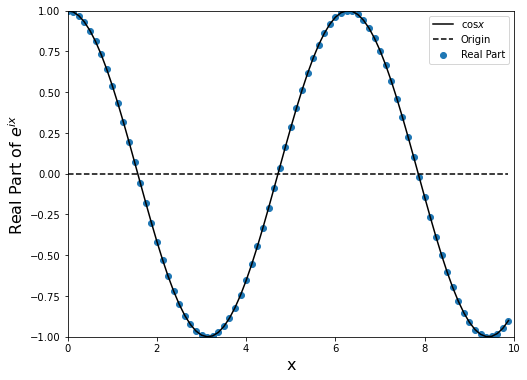
\includegraphics[width=0.7\textwidth, height=0.5\textheight]{img/real.png}
        \caption{\label{fig:real}Real Part $f(x)$ of $e^{ix}$ together with $\cos(x)$}
    \end{figure}
\end{frame}

\begin{frame}
    \frametitle{Step 4}
    The same is done for $g(x)$ and $\sin{x}$.
        \begin{figure}
        \centering
        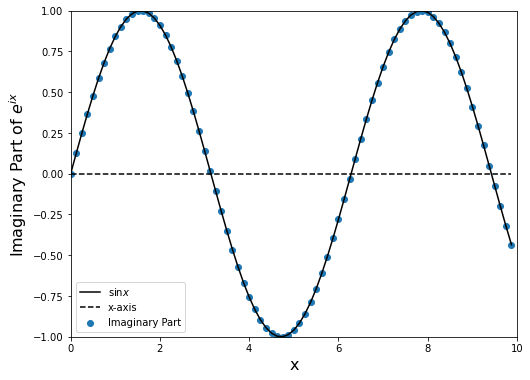
\includegraphics[width=0.7\textwidth, height=0.55\textheight]{img/imaginary.png}
        \caption{\label{fig:imag}Imaginary Part $g(x)$ of $e^{ix}$ together with $\sin(x)$}
    \end{figure}
    \pause
    We can see that $g(x)$ is equivalent to $\sin{x}$.
\end{frame}
\begin{frame}
    Finally I'm plotting the real and imaginary part of $e^{ix}$ together with $\cos{x}$ and $\sin{x}$ on the same axis. The plot shows a perfect fit.
    \begin{figure}
        \centering
        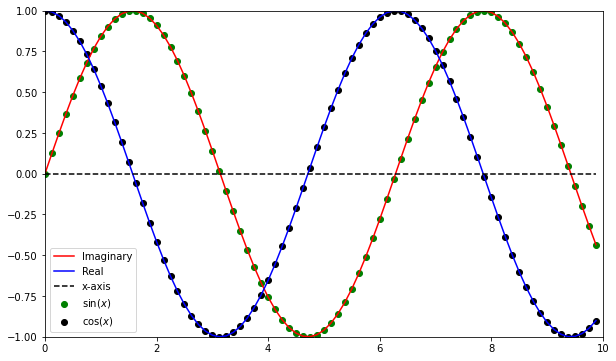
\includegraphics[width=0.7\textwidth]{img/all.png}
        \caption{\label{fig:all}Real and Imaginary Part of $e^{ix}$ together with $\sin(x)$ and $\cos(x)$}
    \end{figure}
\end{frame}

\subsection{Result}
\begin{frame}
    \frametitle{Result}
    By using simple arithmatic and algebra, we generated the tables and plotted their data. We find that even these elementary method gave us one of the most imporatnt relation in complex numbers, namely the Euler's relation:
    \begin{equation*}
            e^{ix} = \cos{x} + i\sin{x}
    \end{equation*}
\end{frame}

\section{Euler's Identity}
\begin{frame}
    \frametitle{Euler's Identity}
    It will be a kind of blasphamy to discuss Euler's equation but leave out Euler's identity given by:
    \begin{equation}
        \label{el-id}
        e^{i\pi} + 1 = 0
    \end{equation}
The equation \ref{el-id} above is considered as \textbf{the most beautiful equation} in Mathematics. The identity can be proved putting $x=\pi$ into Euler's equation \ref{eq:1} So I'm not proving it here.
\end{frame}

\section{References and Links}
\begin{frame}
    \frametitle{References and Links}
    \begin{enumerate}
        \item Feynman's Lectures on Physics
    \end{enumerate}
\end{frame}
\end{document}